% Name: Hexagon equation
% Description: Moving a past b and c on a regular hexagon: braiding with bc at once (R) agrees with braiding past b and then c, with associators F between.
% Tags: hexagon equation, R-move, braiding, coherence

\usetikzlibrary{arrows.meta}

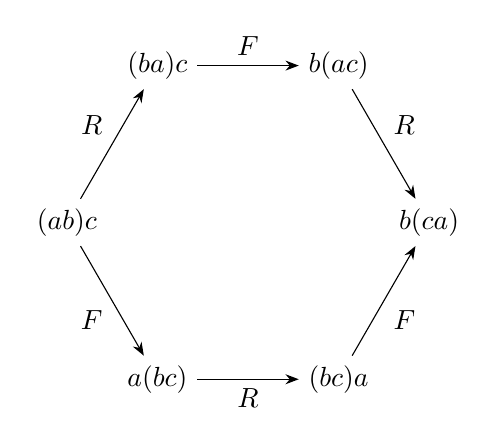
\begin{tikzpicture}[>={Stealth}]
  \node (A) at (180:2.3) {$(ab)c$};
  \node (B) at (120:2.3) {$(ba)c$};
  \node (C) at (60:2.3)  {$b(ac)$};
  \node (D) at (0:2.3)   {$b(ca)$};
  \node (E) at (240:2.3) {$a(bc)$};
  \node (F) at (300:2.3) {$(bc)a$};
  \draw[->] (A) -- node[above left]  {$R$} (B);
  \draw[->] (B) -- node[above]       {$F$} (C);
  \draw[->] (C) -- node[above right] {$R$} (D);
  \draw[->] (A) -- node[below left]  {$F$} (E);
  \draw[->] (E) -- node[below]       {$R$} (F);
  \draw[->] (F) -- node[below right] {$F$} (D);
\end{tikzpicture}
